\documentclass{article}

\usepackage[margin=1in]{geometry}
\usepackage{amsmath,amssymb}
\usepackage[table,xcdraw]{xcolor}
\usepackage{graphicx}
\usepackage{caption}
\usepackage{subcaption}

\graphicspath{ {ReportImages/OneClassSVM/} }


\begin{document}

\title{Autonomous Agents\\
Assignment 2: \emph{Single Agent Learning}}
\author{
Artur Alkaim -- 10859368\\
Peter Dekker -- 10820973\\
Rafael Reia -- 10859454\\
Yikang Wang -- 10540288\\
}
\maketitle
\section{Introduction}
In this assignment, we study the application of \emph{reinforced learning
algorithms}. The main focus of this study is on the Q-Learning algorithm where
we used a \epsilon-policy at the begining and changed other policies to experiment
the efects of that.

Our goal is to tune the algorithms with the different parameters and understand
how this parameters affect the performance that in this specific instance is
determined by the number of steps the predator needs to catch the prey and how
we can improve that with learning. 

\section{Program design}
In this assignment the overall progam design stays the same, as we just added
the equivalent classes for the new algorithms. So we have a new main class,
\emph{MainQl} that, like the others, create a specific environment for the
predator and prey to live. Then it runs the simulation for that setup.

We also added some utility classes to produce the graphs for this report.

\section{Evaluation}

%- Why? 'In order to test\ldots'
%- How? ' we run \ldots N times on X computer'
%- What does it show?
%- Take home message

In order to test how the Q-learning algorithm works with different parameters we
have run our implemetation and computed the average of $100$ runs, each of them
with $10000$ episodes. With the averaging we have been able to get less sharper
graphs.

\subsection{Different learning rates ($\alpha$)}
In order to test the influence of $\alpha$ we run our implementation with
different values. The values used are:
$0.1 , 0.2, 0.3, 0.4 and 0.5$. 

We have noticed that, as expected, when we increse the value of $\alpha$
algorithm converges faster to an optimal value. This happens because this makes the agent
consider the the known information. If we choose $0$ for $\alpha$ the agent
would not learn anything as he would just use the old(inital) values.

In theory we could put it to $1$ to maximise de learning rate, but as our
transitions are not deterministic, because the agent doesn't control the
movement of the prey we can't trust only on learning.

Thus, we should set the values as high as possible but considering this tradeof.
So, as said we used the values from $0.1, \ldots , 0.5$ test and the results are
better with $0.5$ as the chart shows. They all converge but with higher values
they converge faster. The average value shows how fast they converge, because if
a line converge faster, the number of low values will be high and this have a
direct impact on the average.

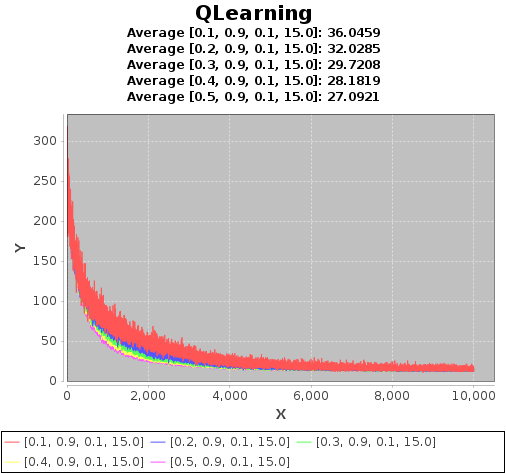
\includegraphics[]{res/alpha_01_to_05_gama_09_epsilon_01_IV_15.png}

\subsection{Different discount factors ($\gamma$)}
We started to experiment with different values of $\gamma$. The values used are:
$0.2, 0.5, 0.7 and 0.9$. 

The discount factor influences the importance that is given to future rewards.
This means that the lower the value, the less the agent cares about future
rewards and considers more the imediate reward. In the limit, if it's set to
$0$ (zero), the agent only considers the imediate reward.

In this problem instance the imediate reward is almost allways zero, so if we
have low $\gamma$ the learned values will be close to zero, i. e., it will not
learn anything. 

Thus, we noticed that by incresing $\gamma$ the number of steps converge to
lower values but don't have a big impact on the convegence rate.

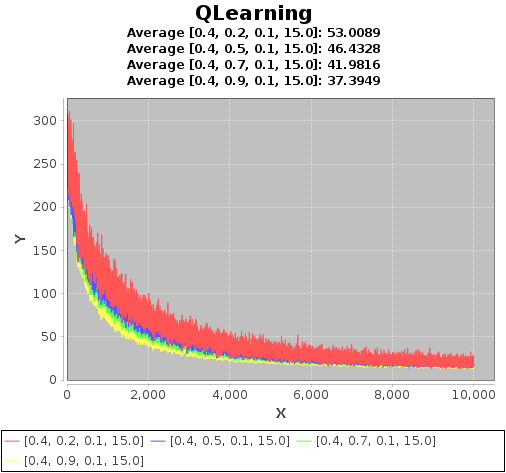
\includegraphics[]{res/alpha_04_gama_02_to_09_epsilon_01_IV_15.png}

The chart shows what we just mentioned, that with higher values for $\gamma$,
the line converges to a lower point.

\subsection{Different Initial Values}
We started to experiment with different values of IV. The values used are:
$0, 1, 15 and 50$. 

As Q-learning is an iterative process, and we assign initial values for the
states, we have to consider what values we use and the impact it may have on the
performance/evolution of the process.

It have been shown that high values for the initialization, aka \"optimistic
initial conditions\", can encourage exploration. This is positive because after
the agent explores all the states and assign the values for that states, in can
start optimizing paths.
With low initial values, consequently low exploration, the number of states that
still have the initial values are higher through the process and when the agent
is surrounded by states with the same value, it chooses randomly. This causes a
behaviour closer to a random policy at the begining cousing the first group of
iterations to have much higher number of steps than with \"optimistic
initial conditions\".

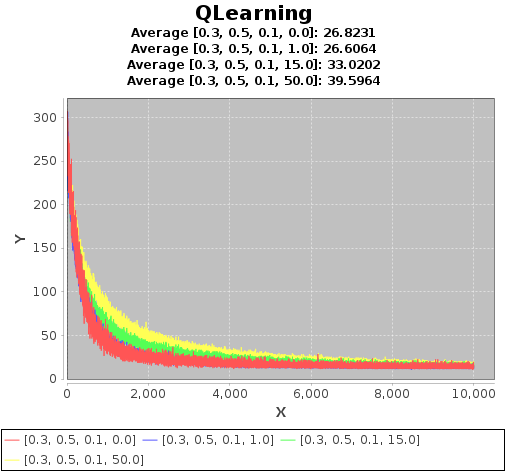
\includegraphics[]{res/alpha_03_gama_05_epsilon_01IV_00_to_50.png}

\section{Policy}
The main policy used was the $\epsilon-greedy$ policy. And with that we had to
tune the value of $\epsilon$ and the results of that tuning are in the following
subsection.

After that we implemented a different policy, softmax policy that is also
described in the subsection \ref{softmax}.

\subsection{Different \epsilon's}
In order to understand the impact of $\epsilon$ to our implementation we run
in with the following values:
$0.1, 0.3, 0.5 and 0.7$.

The $\epsilon$ is a parameter of the $\epsilon-greedy$ policy and not directly
from the Q-Learning algorithm. So this testing shows more how the choosen policy can
influence the learning process and its outcomes. 

As this parameter is related to the probability of choosing a random action over
the higher value action it is another factor of exploration/exploitation
(??????????????????????).

So if the $\epsilon$ is increasd, the the behaviour is again closer to a random
policy, but contrary to what happens with the initial values, this policy have
impact throughout the process and not just at the beginning.

This causes a worst final value after convergence as show in the following
chart.

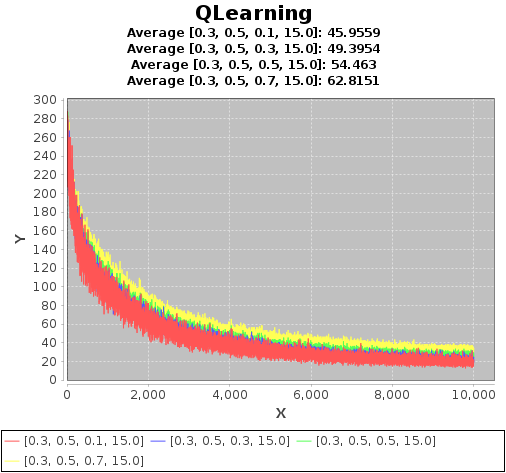
\includegraphics[]{res/alpha_03_gama_05_epsilon_01_to_07_IV_15.png}

\subsection{Softmax}
\label{softmax}

This policy calculates the probablities for each action to be choosed at each
timestamp. This algorithm can be tuned through the parameter $\tau$ that is
caled \emph{temperature}.
The temperature it's a positive value that have impact in the result of the
formula.

With high $\tau$ the probability of all actions are (nearly) the same, causing
this to have a nearly random behaviour.

As $\tau \rightarrow 0$ the behaviour is the same as the $\epsilon-greedy$
policy.
So this policy works with this tradeof, trying to balance totaly random choices
with pure greedy approach.

In our results, softmax have a better/worst(??????????????????????) performance
than the $\epsilon-greedy$ policy.The results presented in the graph shows that
with higher $\tau$ the number of steps is higher, as expected, caused by the
nearly random behaviour.

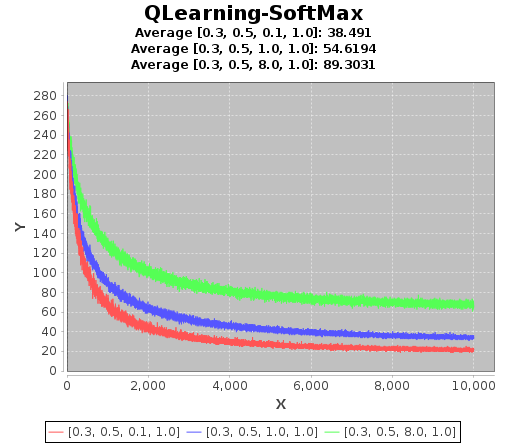
\includegraphics[]{res/alpha_03_gamma_05_temp_01_to_10_IV_1.png}

\section{Conclusion}



\end{document}
